\documentclass[compress]{beamer} 
\usepackage{amsmath,amsthm,amsfonts}
\usepackage{graphicx,microtype,parskip}
\usepackage{caption,subcaption,multirow}
\usepackage{attrib}
\usepackage{appendixnumberbeamer} 

\frenchspacing

\usetheme{default}
\usecolortheme{whale}

\setbeamertemplate{navigation symbols}{}

\setbeamercolor{title}{fg=blue,bg=white}

\setbeamercolor{block title}{fg=white,bg=gray}
\setbeamercolor{block body}{fg=black,bg=lightgray}

\setbeamercolor{block title alerted}{fg=white,bg=darkgray}
\setbeamercolor{block body alerted}{fg=black,bg=lightgray}

\let\Tiny\tiny% http://tex.stackexchange.com/q/58087/5764


% table of contents and subsections
\AtBeginSection[]
{
  \begin{frame}
    \tableofcontents[currentsection]
  \end{frame}
}
\AtBeginSubsection[]
{
  \begin{frame}
    \tableofcontents[currentsection,currentsubsection]
  \end{frame}
}

% boxes prettier
\usepackage{etoolbox}
\newcommand{\zerodisplayskips}{%
  \setlength{\abovedisplayskip}{0pt}%
  \setlength{\belowdisplayskip}{0pt}%
  \setlength{\abovedisplayshortskip}{0pt}%
  \setlength{\belowdisplayshortskip}{0pt}}
  %\appto{\normalsize}{\zerodisplayskips}
  %\appto{\small}{\zerodisplayskips}
  %\appto{\footnotesize}{\zerodisplayskips}


\useoutertheme{infolines}
\usefonttheme[onlymath]{serif}
\setbeamertemplate{headline}[default]
\setbeamertemplate{navigation symbols}{}
\setbeamercovered{transparent}
\setbeamercolor{block body example}{fg=blue, bg=black!20}

\useoutertheme[subsection=false]{miniframes}




\title{Evolutionary macroecology}
\subtitle{modeling emergent patterns in the fossil record}
\author{Peter D Smits}
\institute{Department of Integrative Biology, University of California -- Berkeley}


\begin{document}

\begin{frame}
  \maketitle
\end{frame}

\begin{frame}
  \tableofcontents
\end{frame}

\section[Introduction]{Macroevolution, macroecology, and modeling emergence}

\begin{frame}
  \frametitle{Species response in context}
  
  \begin{center}
    \includegraphics[height=0.8\textheight,width=\textwidth,keepaspectratio=true]{figure/blois_response}
  \end{center}
  \tiny{\attrib{Blois and Hadly, 2009, \em{Annu. Rev. Earth Planet. Sci.}}}
\end{frame}

\begin{frame}
  \begin{columns}
    \begin{column}{0.5\textwidth}
      \begin{center}
        \includegraphics[height=0.8\textheight,width=\textwidth,keepaspectratio=true]{figure/stanley_macro}
      \end{center}
    \end{column}
    \begin{column}{0.5\textwidth}
      \begin{center}
        \includegraphics[height=0.8\textheight,width=\textwidth,keepaspectratio=true]{figure/brown_macro}
      \end{center}
    \end{column}
  \end{columns}
\end{frame}

\begin{frame}
  \frametitle{Core disciplines}
  \begin{definition}
    \begin{itemize}
      \item \alert{macroevolution}: study of patterns which emerge when considering the evolutionary history of multiple species
      \item \alert{macroecology}: study of patterns which emerge when considering the ecology of multiple species
      \item \emph{in both time and space}
    \end{itemize}
  \end{definition}
\end{frame}

\begin{frame}
  \frametitle{Species fitness}

  \begin{alertblock}{Cooper 1984 \em{J. Theoretical Biology}}
    Expected time till extinction.
  \end{alertblock}


  \begin{itemize}
    \item \alert{logic:} if more fit, more likely to be present
    \item distribution based definition (population)
    \item other definitions can be derived based on definition of extinction
  \end{itemize}
\end{frame}

\begin{frame}
  \frametitle{Species selection}

  \begin{alertblock}{Rabosky and McCune 2010 \em{TREE}}
    \begin{quote}
      Species selection is the outcome of heritable variation in speciation and extinction rates among taxa.
    \end{quote}
  \end{alertblock}

  \begin{itemize}
    \item non-operational definition; describes phenomenon
    \item avoids selection versus sorting, \\``strict'' species selection versus effect macroevolution
  \end{itemize}
\end{frame}

\begin{frame}
  \frametitle{Traits as conceptual and operational link}

  \begin{definition}
    \begin{itemize}
      \item \alert{trait}: identifiable property of an organism \\e.g. pelage color, body mass, beak depth, tooth shape
      \item \alert{functional trait}: trait that strongly influences performance/means of interacting with environment
      \item \alert{species trait}: identifiable property assignable to a species
    \end{itemize}
  \end{definition}
\end{frame}

\begin{frame}
  \frametitle{Structured data in biology and paleontology}

  \begin{center}
    \includegraphics[width = \textwidth,height = 0.75\textheight,keepaspectratio = true]{figure/ovaskainen_data}
  \end{center}

  \tiny{\attrib{Ovaskainen \textit{et al.} 2017 \em{Ecology Letters}}}
\end{frame}

\begin{frame}
  \frametitle{Models of structured data}

  \begin{center}
    \includegraphics[width = \textwidth,height = 0.8\textheight,keepaspectratio = true]{figure/ovaskainen_dag}
  \end{center}

  \tiny{\attrib{Ovaskainen \textit{et al.} 2017 \em{Ecology Letters}}}
\end{frame}

\begin{frame}
  \begin{center}
    \includegraphics[width = \textwidth,height = 0.8\textheight,keepaspectratio = true]{figure/han_bayes}
  \end{center}

  \tiny{\attrib{www.countbayesie.com}}
\end{frame}

\begin{frame}
  \frametitle{Parameter estimation and inference}
  \begin{columns}
    \begin{column}{0.45\textwidth}
      \begin{itemize}
        \item \textbf{Bayesian inference}
          \begin{itemize}
            \item intuitive, expressive
            \item regularization
            \item external information
          \end{itemize}
        \item Hamiltonian Monte Carlo/NUTS
          \begin{itemize}
            \item fewer samples/greater ESS vs Gibbs etc.
          \end{itemize}
        \item Automatic Differentiation Variational Inference (ADVI)
          \begin{itemize}
            \item when full HMC/MCMC slow
            \item approximate posterior as Gaussian
          \end{itemize}
      \end{itemize}
    \end{column}
    \begin{column}{0.55\textwidth}
      \begin{center}
        \includegraphics[height=0.7\textheight,width=\textwidth,keepaspectratio=true]{figure/stan_logo}

        \vspace*{0.05\textheight}

        \LARGE{\textbf{Stan}}
      \end{center}
    \end{column}
  \end{columns}
\end{frame}



%\begin{frame}
%  \frametitle{Mammals and brachiopods}
%
%  \begin{columns}
%    \begin{column}{0.5\textwidth}
%      \begin{center}
%        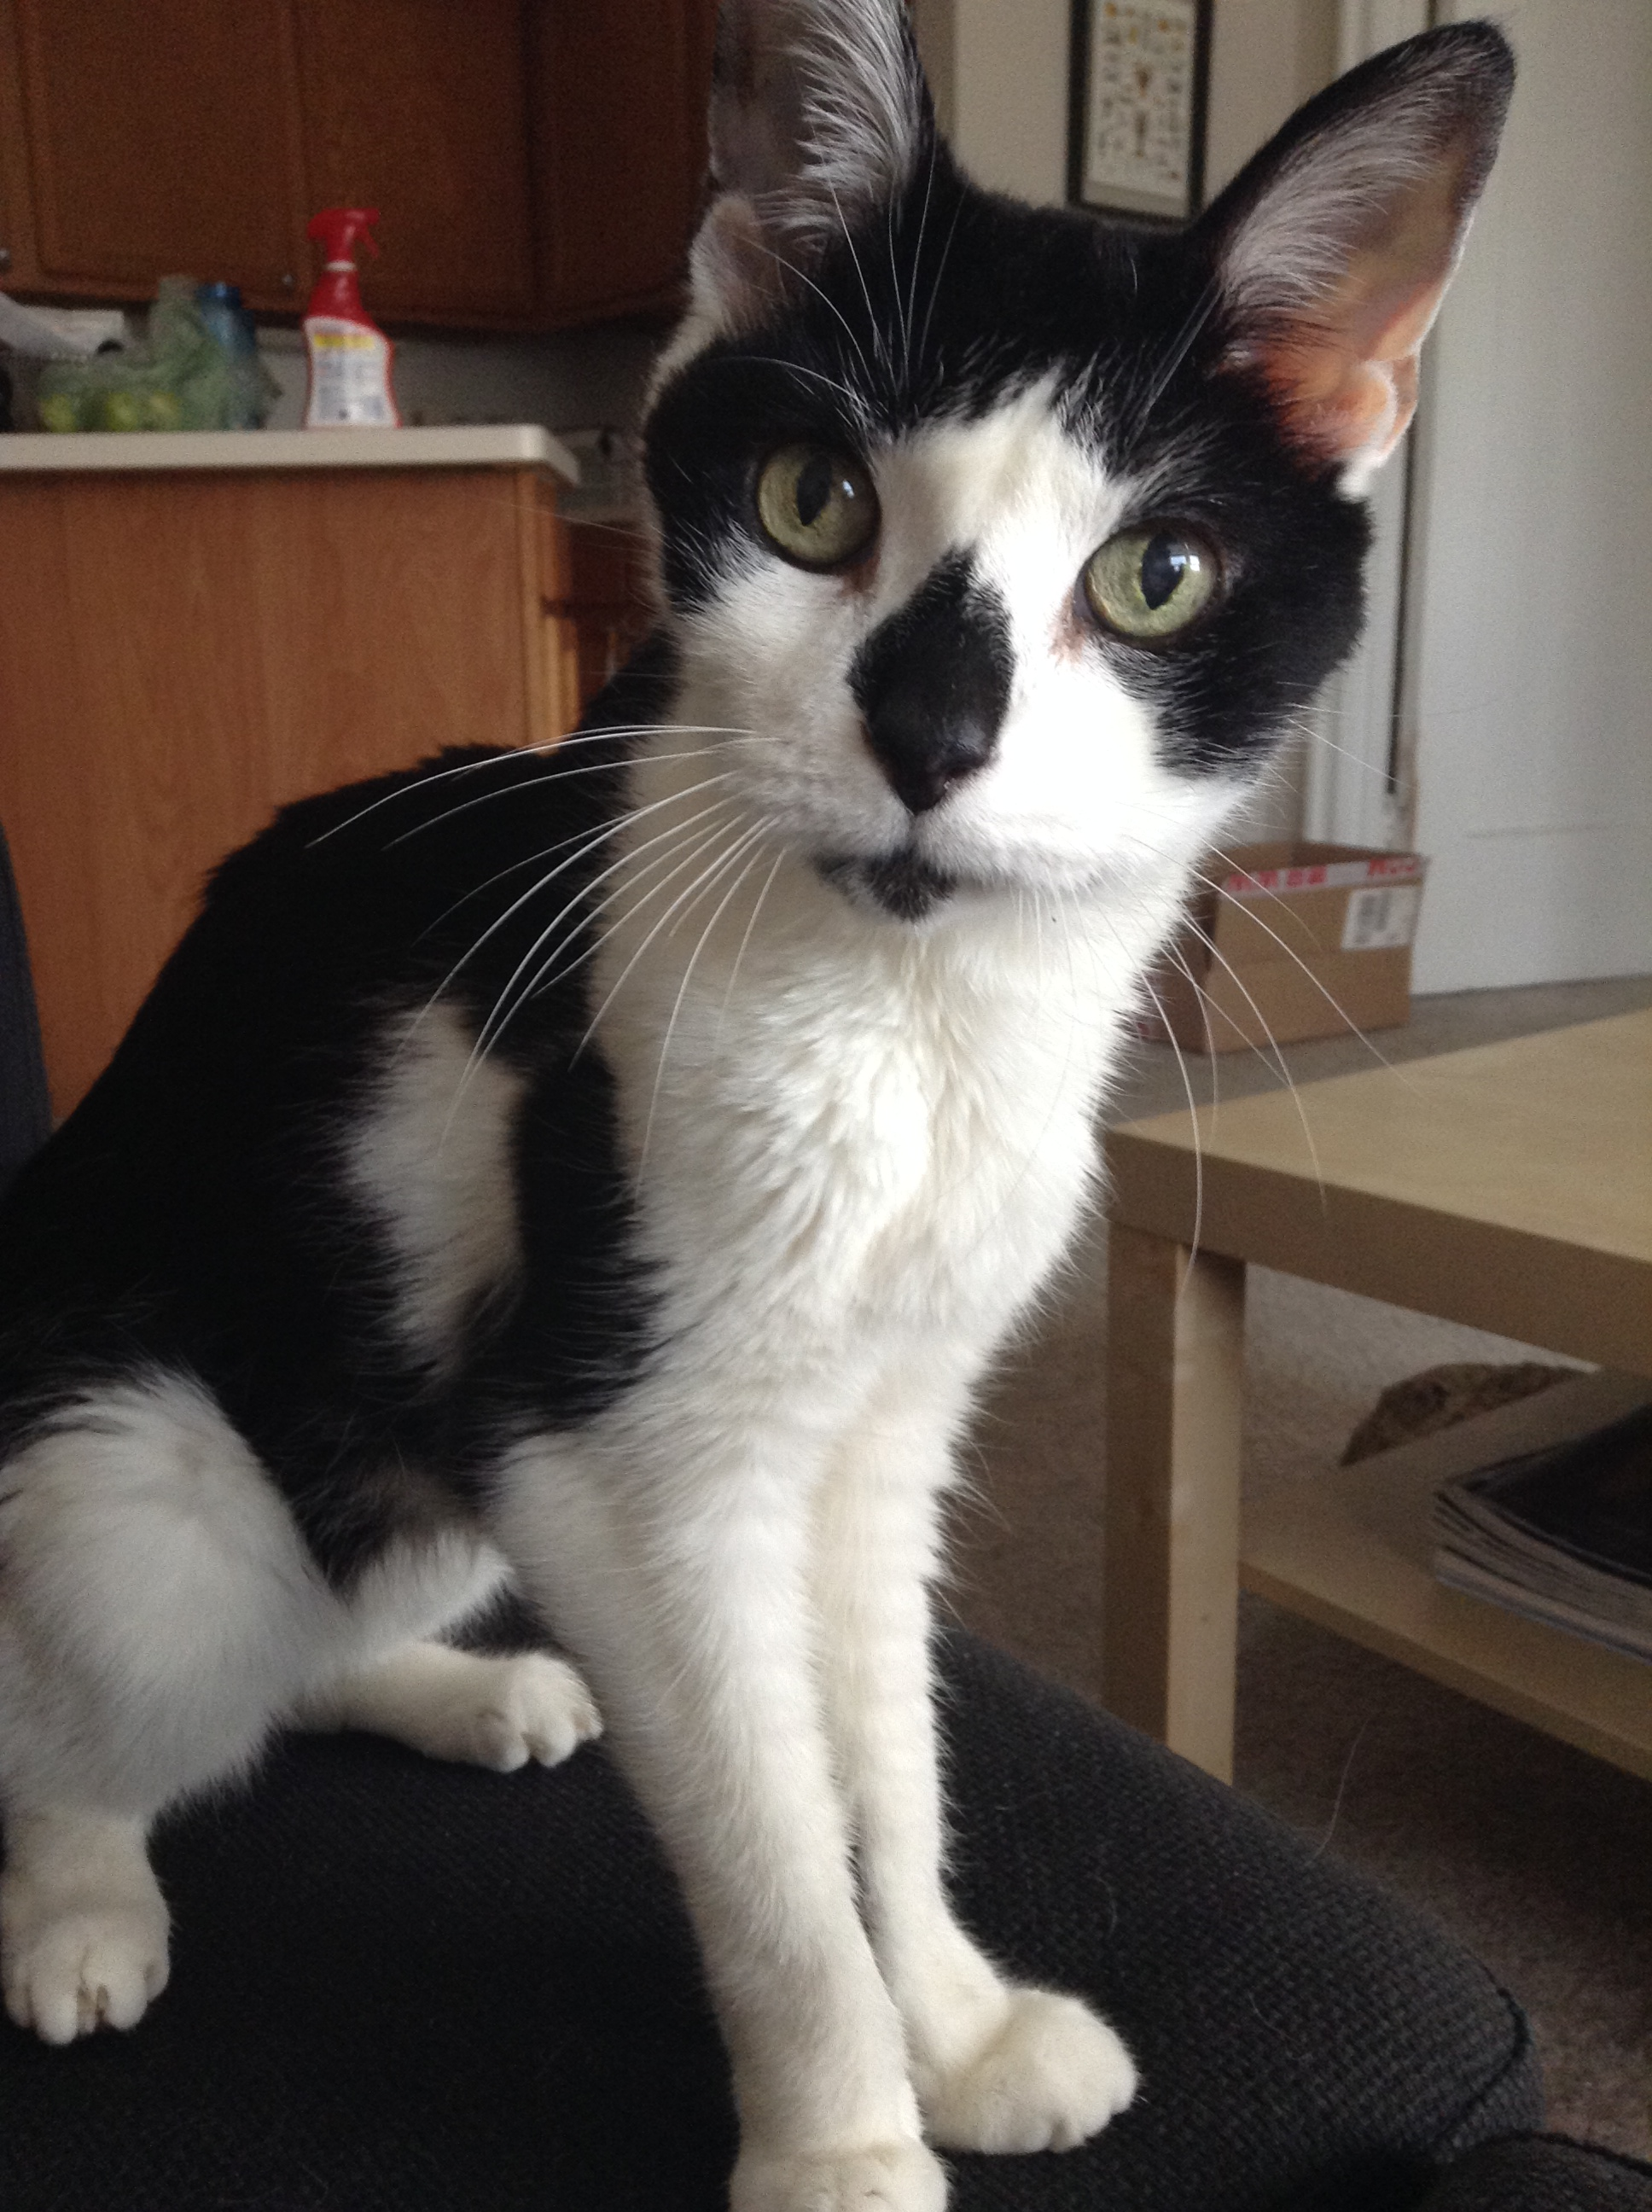
\includegraphics[height = 0.6\textheight, keepaspectratio = true]{figure/monty}
%      \end{center}
%    \end{column}
%    \begin{column}{0.5\textwidth}
%      \begin{center}
%        \includegraphics[height = 0.6\textheight, keepaspectratio = true]{figure/tattoo}
%      \end{center}
%    \end{column}
%  \end{columns}
%\end{frame}



\section[Mammal survival]{Mammal species survival as function of ecology and history}


\begin{frame}
  \begin{alertblock}{Motivating questions}
    \begin{itemize}
      \item How do mammal species traits affect extinction risk?
        \begin{itemize}
          \item How do shared time of origination or evolutionary history relate to extinction risk?
        \end{itemize}
      \item How do my findings compare to current risk factors?
      \item Is species extinction risk age-independent?
    \end{itemize}
  \end{alertblock}
\end{frame}

\begin{frame}
  \frametitle{Extinction}
  \begin{block}{Simpson 2016 \em{bioRxiv}}
    \begin{quote}
      Population decline maybe a common cause of \dots extinction, but organisms never die from population decline, and population decline is never caused by organismal death alone \dots It's the relative balance between birth, death, and lifespan of organisms that determines \dots extinction. 
    \end{quote}
  \end{block}
\end{frame}

%\begin{frame}
%  \frametitle{Law of Constant Extinction}
%
%  \begin{block}{Van Valen 1973 \em{Evol. Theory}}
%    Extinction risk (species fitness), in a given adaptive zone, is taxon--age independent.
%  \end{block}
%
%  \begin{center}
%    \includegraphics[width = \textwidth,height = 0.5\textheight,keepaspectratio = true]{figure/surv_sim}
%  \end{center}
%\end{frame}

\begin{frame}
  \frametitle{Survival of the unspecialized}
  \begin{block}{Simpson 1944 \em{Tempo and Mode in Evolution} p. 143}
    \begin{quote}
      When related phyla die out \dots more specialized phyla tend to become extinct before less specialized. This phenomenon is also far from universal, but it is so common that it does deserve recognition as a rule or principle in evolutionary studies: \textbf{the rule of the survival of the relatively unspecialized.}
    \end{quote}
  \end{block}
\end{frame}

\begin{frame}
  \frametitle{Age of Mammals}
  \begin{center}
    \includegraphics[width = \textwidth,height = 0.8\textheight,keepaspectratio = true]{figure/aom}
  \end{center}

  \tiny{\attrib{Rudolph Zallinger}}
\end{frame}

\begin{frame}
  \frametitle{Relationship between range size and extinction risk}
  \begin{center}
    \includegraphics[width = \textwidth,height = 0.8\textheight,keepaspectratio = true]{figure/geo_range_1}
  \end{center}
\end{frame}

\begin{frame}
  \frametitle{Relationship between range size and extinction risk}
  \begin{center}
    \includegraphics[width = \textwidth,height = 0.8\textheight,keepaspectratio = true]{figure/geo_range_2}
  \end{center}
\end{frame}

\begin{frame}
  \frametitle{Hypotheses of effects of locomotor category}
  \begin{center}
    \includegraphics[width = \textwidth,height = 0.8\textheight,keepaspectratio = true]{figure/loco_initial}
  \end{center}
\end{frame}

\begin{frame}
  \frametitle{Hypotheses of effects of locomotor category}
  \begin{center}
    \includegraphics[width = \textwidth,height = 0.8\textheight,keepaspectratio = true]{figure/loco_later}
  \end{center}
\end{frame}

\begin{frame}
  \frametitle{Hypotheses of effects of dietary category}
  \begin{center}
    \includegraphics[width = \textwidth,height = 0.8\textheight,keepaspectratio = true]{figure/diet_survival}
  \end{center}
\end{frame}

\begin{frame}
  \frametitle{Survival model diagram}
  \begin{center}
    \includegraphics[height=0.8\textheight,keepaspectratio=true]{figure/mammal_survival_model}
  \end{center}
\end{frame}

\begin{frame}
  \frametitle{Pattern of species survival under two models}

  \begin{center}
    \includegraphics[height=0.75\textheight,keepaspectratio=true]{figure/survival_function_pres}
  \end{center}

  \tiny{\attrib{Smits 2015 \em{PNAS}}}
\end{frame}

\begin{frame}
  \frametitle{Effect of locomotor category on extinction risk}

  \begin{center}
    \includegraphics[height=0.75\textheight,keepaspectratio=true]{figure/loco_diff_est}
  \end{center}

  \tiny{\attrib{Smits 2015 \em{PNAS}}}
\end{frame}

\begin{frame}
  \frametitle{Effect of dietary category on extinction risk}

  \begin{center}
    \includegraphics[height=0.8\textheight,keepaspectratio=true]{figure/diet_diff_est}
  \end{center}

  \tiny{\attrib{Smits 2015 \em{PNAS}}}
\end{frame}

\begin{frame}
  \frametitle{Difference in risk between origination cohorts}

  \begin{center}
    \includegraphics[height=0.8\textheight,keepaspectratio=true]{figure/cohort_est_pres}
  \end{center}

  \tiny{\attrib{Smits 2015 \em{PNAS}}}
\end{frame}

\begin{frame}
  \frametitle{Three sources of variance}

  \begin{center}
    \includegraphics[height=0.8\textheight,keepaspectratio=true]{figure/variance_est}
  \end{center}

  \tiny{\attrib{Smits 2015 \em{PNAS}}}
\end{frame}

\begin{frame}
  \begin{block}{Summary of results}
    \begin{itemize}
      \item survival of the unspecialized as time-invariant generalization
      \item decrease in extinction risk towards the present
        \begin{itemize}
          \item both cohort/temporal and phylogenetic effect
        \end{itemize}
      \item accelerating extinction risk with age (not discussed)
      \item no effect of mass on survival (not discussed)
      \item some incongruence with risk factors in the Recent
        \begin{itemize}
          \item e.g. effect of body size, trophic category, phylogenetic clustering
        \end{itemize}
    \end{itemize}
  \end{block}
\end{frame}



\section[Functional diversity]{Changes to the functional diveristy of the NA mammal species pool}

\begin{frame}
  \begin{alertblock}{Question}
    \alert{Why} do the relative diversities of functional groups change within a species pool?
    \begin{itemize}
      \item function of \alert{species traits} and \alert{environmental context}
    \end{itemize}
  \end{alertblock}
\end{frame}

\begin{frame}
  \frametitle{Eco-cube and functional groups}

  \begin{center}
    \includegraphics[height=0.8\textheight,width=\textwidth,keepaspectratio=true]{figure/bush_cube_time}
  \end{center}

  \tiny{\attrib{Bush and Bambach 2011 \em{Annu. Rev. Earth Planet Sci.}}}
\end{frame}

\begin{frame}
  \frametitle{Species pool concept}

  \begin{center}
    \includegraphics[height=0.8\textheight,width=\textwidth,keepaspectratio=true]{figure/schemske_pool}
  \end{center}

  \tiny{\attrib{Mittelbach and Schemske, 2015, \em{TREE}}}
\end{frame}

\begin{frame}
  \frametitle{Cenozoic mammals of North America}
  \begin{center}
    \includegraphics[height=0.8\textheight,width=\textwidth,keepaspectratio=true]{figure/aom}
  \end{center}

  \tiny{\attrib{Rudolph Zallinger}}
\end{frame}

\begin{frame}
  \frametitle{Conceptualizing the knowns and unknowns}
  \begin{center}
    \includegraphics[width=0.9\textwidth,height=\textheight,keepaspectratio=true]{figure/problem_concept}
  \end{center}
\end{frame}

\begin{frame}
  \frametitle{Covariates of interest, temporal structure}

  \begin{center}
    \large{species occurrence (\(\sim\)1400 species) by NALMA}
  \end{center}

  \vspace*{0.05\textheight}

  \begin{columns}
    \begin{column}[T]{0.5\textwidth}
      \textbf{functional group}
      \begin{itemize}
        \small{
        \item dietary category: \\\begin{tiny}carnivore, herbivore, insectivore, omnivore\end{tiny}
        \item locomotor category: \\\begin{tiny}arboreal, digitigrade, fossorial, plantigrade, scansorial, unguligrade\end{tiny}
        }
      \end{itemize}
  
      \vspace*{0.01\textheight}

      \textbf{observation}
      \begin{itemize}
        \item indiv-level: species
          \begin{itemize}
            \small{
            \item functional group
            \item mean mass
            }
          \end{itemize}
        \item time of observation
      \end{itemize}
    \end{column}
    \begin{column}[T]{0.5\textwidth}
      \textbf{origination and survival}
      \begin{itemize}
        \item indiv-level: species
          \begin{itemize}
            \small{
            \item functional group
            \item taxon order
            \item mean mass
            }
          \end{itemize}
        \item group-level: FG/time
          \begin{itemize}
            \small{
            \item temperature est Mg/Ca \\ 
              \begin{tiny}
                Cramer \em{et al.}, 2011, J. Geophy. Res.
              \end{tiny}
            \item plant phase (Pa-Eo, Eo-Mi, Mi-Pl) \\ 
              \begin{tiny}
                Graham, 2011, \underline{A natural history of the New World}
              \end{tiny}
            }
          \end{itemize}
      \end{itemize}
    \end{column}
  \end{columns}
\end{frame}

\begin{frame}
  \frametitle{Conceptualizing the analysis}
  \begin{center}
    \includegraphics[width=0.9\textwidth,height=\textheight,keepaspectratio=true]{figure/paleo_fourth_corner}
  \end{center}
\end{frame}



\begin{frame}
  \frametitle{Origination; individual-level}
  \begin{center}
    probability of species originating, given it hasn't originated yet

    \includegraphics[height=0.8\textheight,width=\textwidth,keepaspectratio=true]{figure/ecotype_origin_bd}
  \end{center}
\end{frame}

\begin{frame}
  \frametitle{Origination; group-level}
  \begin{center}
    change to log-odds of species originating, given it hasn't originated yet

    \includegraphics[height=0.8\textheight,width=\textwidth,keepaspectratio=true]{figure/group_on_origin_bd}
  \end{center}
\end{frame}

\begin{frame}
  \frametitle{Survival; individual-level}
  \begin{center}
    probability of species surviving, given it was present

    \includegraphics[height=0.8\textheight,width=\textwidth,keepaspectratio=true]{figure/ecotype_survival_bd}
  \end{center}
\end{frame}

\begin{frame}
  \frametitle{Survival; group-level}
  \begin{center}
    change to log-odds of species surviving, given it was present

    \includegraphics[height=0.8\textheight,width=\textwidth,keepaspectratio=true]{figure/group_on_survival_bd}
  \end{center}
\end{frame}

\begin{frame}
  \frametitle{Relative diversity of functional groups through time}
  \begin{center}
    \includegraphics[height=0.9\textheight,width=\textwidth,keepaspectratio=true]{figure/relative_diversity}
  \end{center}
\end{frame}

\begin{frame}
  \begin{block}{Changes to relative diversity between Neogene/Paleogene}
    \begin{itemize}
      \item \alert{increase}
        \begin{itemize}
          \item digitigrade, plantigrade, unguligrade herbivores
          \item fossorial functional groups
          \item plantigrade omnivores
        \end{itemize}
      \item \alert{decrease}
        \begin{itemize}
          \item near total loss of arboreal functional groups
          \item plantigrade, scansorial insectivores
          \item unguligrade omnivores
        \end{itemize}
    \end{itemize}
  \end{block}
\end{frame}

\begin{frame}
  \begin{alertblock}{Conclusions}
    \begin{itemize}
      \item time has larger effect on P(observation) than FG 
      \item increase P(origination), decrease P(survival) but not always 
      \item environmental affect FG origination more than survival
      \item no evidence for correlation btwn FG origination or survival
        \begin{itemize}
          \item potential short-term links, but no long-term correlation
        \end{itemize}
      \item HMC/MCMC might tweak these results b/c ADVI assumptions
    \end{itemize}
  \end{alertblock}
\end{frame}




\section[Fossil/Not Fossil]{Fossil/Not Fossil and grappling with facies shift, truncation, geography}

\begin{frame}
  \frametitle{In what rocks can we expect to see fossils?}
  \begin{itemize}
    \item \alert{to find a fossil we first need to find a ``good rock''}
    \item what properties can we use to define a ``good rock''?
    \item what is the expected number of fossil species when there are no ``good rocks''?
  \end{itemize}
\end{frame}

\begin{frame}
  \frametitle{Why worry about losing ``good rocks''?}
  \begin{center}
    \includegraphics[height=0.8\textheight,width=\textwidth,keepaspectratio=true]{figure/peters_common_cause}
  \end{center}
  
  \tiny{\attrib{Peters, 2008, \em{Nature}}}
\end{frame}


\begin{frame}
  \frametitle{Why worry about losing ``good rocks''?}
  \begin{columns}
    \begin{column}{0.5\textwidth}
      \begin{center}
        \includegraphics[height=0.8\textheight,width=\textwidth,keepaspectratio=true]{figure/finnegan_pnas12_1}
      \end{center}
    \end{column}
    \begin{column}{0.5\textwidth}
      \begin{center}
        \includegraphics[height=0.8\textheight,width=\textwidth,keepaspectratio=true]{figure/finnegan_pnas12_2}
      \end{center}
    \end{column}
  \end{columns}
    
  \tiny{\attrib{Finnegan \textit{et al.}, 2012, \em{PNAS}}}
\end{frame}

\begin{frame}
  \frametitle{Ordovician geologic units in Macrostrat}

  \begin{block}{How to describe a geological unit?}
    \begin{itemize}
      \item lithology, percent composition
      \item max, min unit thickness (km)
      \item tropical or temperate at start, finish
      \item km traveled between unit start,stop coordinates
      \item subsurface unit
      \item units above, below
    \end{itemize}
  \end{block}
\end{frame}

\begin{frame}
  \frametitle{Brachiopod counts in Ordovician geologic units}
  \begin{center}
    \includegraphics[height=0.85\textheight,width=\textwidth,keepaspectratio=true]{figure/ordovician_counts}
  \end{center}
\end{frame}


\begin{frame}
  \frametitle{Simulating fossil species from a basic hurdle model}
\begin{equation*}
  p(y | \theta, \lambda)  = 
  \begin{cases}
    \theta & \text{if } y = 0, and \\
    (1 - \theta) \frac{\text{Poisson}(y, \lambda)}{1 - \text{PoissonCDF}(0 | \lambda)} & y > 0
  \end{cases}
\end{equation*}
  \begin{center}
    \includegraphics[height=0.6\textheight,width=\textwidth,keepaspectratio=true]{figure/hurdle_simulation}
  \end{center}
\end{frame}





\begin{frame}
  \frametitle{Acknowledgements}
  \begin{columns}
    \begin{column}{0.5\textwidth}
      \begin{itemize}
        \item UC Berkeley
          \begin{itemize}
            \item \textbf{Seth Finnegan}, \\Adiel Klompmaker, \\Emily Orzechowski, \\Larry Taylor, \\Sara Kahanamoku, \\Josh Zimmt
          \end{itemize}
        \item UChicago
          \begin{itemize}
            \item \textbf{Kenneth D. Angielczyk}, \\\textbf{Michael J. Foote}, \\P. David Polly, \\Richard H. Ree, \\Graham Slater
          \end{itemize}
      \end{itemize}
    \end{column}
    \begin{column}{0.5\textwidth}
      \begin{center}
        \includegraphics[height=0.15\textheight,width=\textwidth,keepaspectratio=true]{figure/github-logo}

        \tiny{psmits.github.io/}
      \end{center}
      \vspace*{0.02\textheight}
      \begin{center}
        \includegraphics[height=0.15\textheight,width=0.5\textwidth,keepaspectratio=true]{figure/twitter} 

        \tiny{@PeterDSmits}
      \end{center}
      \vspace*{0.01\textheight}
      \begin{center}
        \includegraphics[height=0.3\textheight,width=0.5\textwidth,keepaspectratio=true]{figure/paleodb}
        \includegraphics[height=0.25\textheight,width=0.5\textwidth,keepaspectratio=true]{figure/macrostrat}
      \end{center}
    \end{column}
  \end{columns}
\end{frame}


\appendix





\begin{frame}
  \frametitle{Hidden Markov Model with absorbing state}
  \begin{block}{Jolly-Seber CMR/Restricted occupancy model}
    \setlength\abovedisplayskip{-0.3cm}
    \begin{align*}
      y_{i, t} &\sim \text{Bernoulli}(z_{i, t} p_{i, t}) \\
      z_{i, t = 1} &\sim \text{Bernoulli}(\phi_{i, t = 1}) \\
      z_{i, t} &\sim \text{Bernoulli}\left(z_{i, t - 1} \pi_{i,t} + \sum_{x = 1}^{t}(1 - z_{i, x}) \phi_{i, t}\right)
    \end{align*}
    \begin{scriptsize}
      \(y\) observed state; \(z\) estimated state

      \(p\) observation; \(\phi\) origination; \(\pi\) survival

      \(i\) in \(N\); \(t\) in \(T\)
    \end{scriptsize}
  \end{block}
\end{frame}

\begin{frame}
  \frametitle{Modeling the probabilities; individual-level}
  \begin{block}{Multi-level logistic regression}
    \setlength\abovedisplayskip{-0.3cm}
    \begin{align*}
      p_{i, t} &\sim \text{logit}^{-1}(b_{t} + e_{j[i]} + \beta^{p} mass_{i}) \\
      \phi_{i, t} &\sim \text{logit}^{-1}(f^{\phi}_{j[i], t} + o^{\phi}_{k[i]} + \beta^{\phi} mass_{i}) \\
      \pi_{i, t} &\sim \text{logit}^{-1}(f^{\pi}_{j[i], t} + o^{\pi}_{k[i]} + \beta^{\pi} mass_{i})
    \end{align*}
    \begin{scriptsize}
      observation: \(b_{t}\) time-varying intercept; \(e_{j[i]}\) functional group eff; \(\beta^{p}\) mass eff

      origination: \(f^{\phi}_{j[i], t}\) time/FG-varying intercept; \(o^{\phi}_{j[i]}\) order eff; \(\beta^{\phi}\) mass eff

      survival: \(f^{\pi}_{j[i], t}\) time/FG-varying intercept; \(o^{\pi}_{j[i]}\) order eff; \(\beta^{\pi}\) mass eff
    \end{scriptsize}
  \end{block}
\end{frame}

%\gamma^{j = 1}_0 + \gamma^{j = 1}_1 phase_{2} + \gamma^{j = 1}_{2} phase_{3} + \gamma^{j = 1}_{3} temp_{t} \\
\begin{frame}
  \frametitle{Modeling the probabilities; group-level}
  \begin{block}{Multivariate regression of time/FG-varying intercept}
    \setlength\abovedisplayskip{-0.3cm}
    \begin{align*}
      f^{\phi} &\sim \text{MVN}\left(
      \begin{matrix}
        U \gamma^{\phi}_{j = 1} \\
        %U_{t, \_} \gamma^{\phi}_{j = 2} \\
        \vdots \\
        U \gamma^{\phi}_{j = J}
      \end{matrix}, 
      \text{diag}(\tau_{f^{\phi}}) \Omega_{f^{\phi}} \text{diag}(\tau_{f^{\phi}}) \right) \\
      f^{\pi} &\sim \text{MVN}\left(
      \begin{matrix}
        U \gamma^{\pi}_{j = 1} \\
        %U_{t, \_} \gamma^{\pi}_{j = 2} \\
        \vdots \\
        U \gamma^{\pi}_{j = J}
      \end{matrix}, 
      \text{diag}(\tau_{f^{\pi}}) \Omega_{f^{\pi}} \text{diag}(\tau_{f^{\pi}}) \right)
    \end{align*}
    \begin{scriptsize}
      \(U\) matrix group-level covariates; \(\gamma^{\phi}\), \(\gamma^{\pi}\) vectors group-level reg coefs

      \(\Omega_{\phi}\), \(\Omega_{\pi}\) corr matrix of FG by time; \(\tau_{\phi}\), \(\tau^{\pi}\) scale of FG by time
    \end{scriptsize}
  \end{block}
\end{frame}

\begin{frame}
  \frametitle{Modeling the probabilities; final details}

  \begin{block}{Comments on priors, implementation}
    \setlength\abovedisplayskip{-0.1cm}
    \begin{itemize}
      \item random-walk priors on time-varying intercepts
      \item regularizing priors with some specific predictions
        \begin{itemize}
          \item very weak/no effect of mass e.g. \(\mathcal{N}(0, 0.5)\)
          \item very weak/no effect of group-level covariates e.g. \(\mathcal{N}(0, 0.5)\)
          \item very weak/no correlation b/w functional groups e.g. LKJ\((2)\)
        \end{itemize}
      \item marginalization problem b/c gradient based estimation
    \end{itemize}
  \end{block}
\end{frame}

\begin{frame}
  \frametitle{Model adequate? Posterior predictive check}
  \begin{center}
    mean \# occurrences per species from datasets simulated from posterior

    \includegraphics[height=0.8\textheight,width=\textwidth,keepaspectratio=true]{figure/pred_occ_bd}
  \end{center}
\end{frame}

\begin{frame}
  \frametitle{Observation; NALMA}
  \begin{center}
    log-odds of observing a species, given that it is present

    \includegraphics[height=0.8\textheight,width=\textwidth,keepaspectratio=true]{figure/time_observation}
  \end{center}
\end{frame}

\begin{frame}
  \frametitle{Observation; functional group}
  \begin{center}
    log-odds of observing a species, given that it is present

    \includegraphics[height=0.8\textheight,width=\textwidth,keepaspectratio=true]{figure/ecotype_observation}
  \end{center}
\end{frame}


\begin{frame}
  \frametitle{Standing diversity of functional groups through time}
  \begin{center}
    \includegraphics[height=0.9\textheight,width=\textwidth,keepaspectratio=true]{figure/ecotype_diversity}
  \end{center}
\end{frame}

\end{document}
